\begin{surferPage}[Cayley]{Het derdegraadsoppervlak van Cayley}
   Dit oppervlak van graad $3$ heeft in totaal vier singulariteiten die de vorm hebben van een dubbele kegel, zoals het vorige oppervlak.
    Hij is vernoemd naar Arthur Cayley, die veel onderzoek deed naar derdegraadsoppervlakken in de 19de eeuw.
    
    Toch was het Ludwig Schl\"afi die deze oppervlakken in 1863 eerst op systematische manier classificeerde, volgens het aantal singulariteiten dat ze bevatten.
  	In zijn artikel kan je bijvoorbeeld lezen waarom er niet meer dan 4 singuliere punten op zo'n oppervlak kunnen zijn.
    Dit zorgt ervoor dat $\mu(3)=4$. 
    
    Rond het jaar 1900 bestudeerde ook Felix Klein de mogelijke vormen van re\"ele oppervlakken van de derde graad; hij pakte dit aan door kleine vervormingen op het derdegraadsoppervlak van Cayley door te voeren.
    Door de dubbele kegels uit te breiden en delen te scheiden of samen te voegen, slaagde hij erin om alle mogelijke vormen te ontdekken. Hier zien we er enkele: 
    \vspace{0.3cm}
     \begin{center}
      \vspace{-0.2cm}
      \begin{tabular}{@{}c@{\ }c@{\ }c@{\ }c@{}}
        \begin{tabular}{@{}c@{}}
          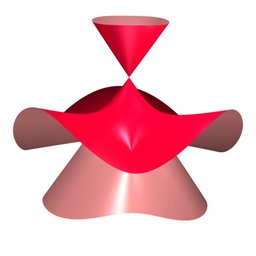
\includegraphics[width=1.35cm]{./../../common/images/cayley_cubic_0}
        \end{tabular}
        &
        \begin{tabular}{@{}c@{}}
          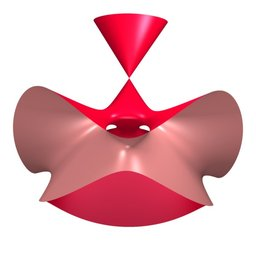
\includegraphics[width=1.35cm]{./../../common/images/cayley_cubic_1}
        \end{tabular}
        &
        \begin{tabular}{@{}c@{}}
          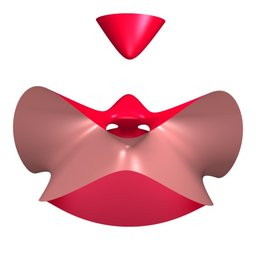
\includegraphics[width=1.35cm]{./../../common/images/cayley_cubic_2}
        \end{tabular}
        &
        \begin{tabular}{@{}c@{}}
          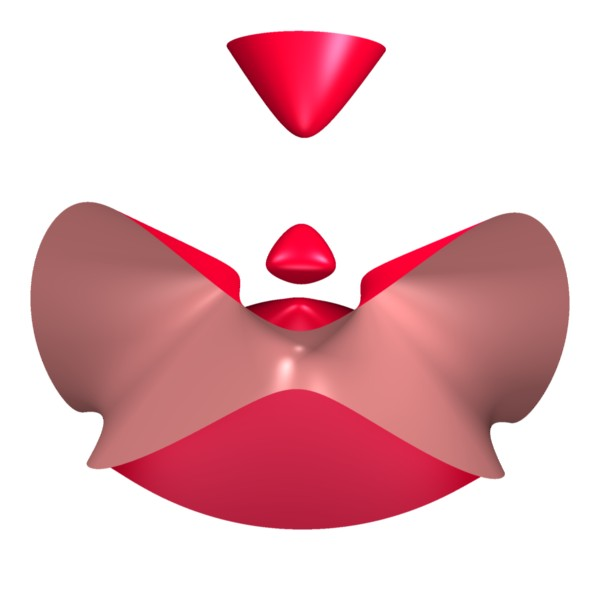
\includegraphics[width=1.35cm]{./../../common/images/cayley_cubic_3}
        \end{tabular}
      \end{tabular}
    \end{center}
\end{surferPage}
